% === C02 - Modo Protegido ===
% David Alejandro Gonzalez Marquez
% dmarquez@dc.uba.ar / fokerman@gmail.com
% https://github.com/fokerman/Orga2Course

\documentclass[aspectratio=169]{beamer}
% \documentclass[handout]{beamer}

% % % Packages
\usepackage[sfdefault]{AlegreyaSans}
\usepackage{inconsolata}
\usepackage{multicol}
\usepackage{multirow}
\usepackage[spanish]{babel}
\usepackage[utf8]{inputenc}
\usepackage{enumerate}
\usepackage{color}
\usepackage{xcolor}
\usepackage[absolute,overlay]{textpos}
  \setlength{\TPHorizModule}{1mm}
  \setlength{\TPVertModule}{1mm}
\usepackage{framed}
\usepackage{mfirstuc} % para poner en mayusculas la primer letra
\usepackage{xspace} % para crear espacios en comandos 
\usepackage{pbox}
\usepackage{tikz}
\usepackage{mathabx}

% % % Beamer config
\usetheme{Pittsburgh}
\usecolortheme[rgb={1,0.48,0.0}]{structure}
\setbeamercolor{block title}{fg=white,bg=verdeuca}
\xdefinecolor{verdeuca}{rgb}{0.0,0.48,0.54}
\xdefinecolor{naranjauca}{rgb}{1,0.48,0.0}
\setbeamercolor{palette quaternary}{fg=white,bg=verdeuca}
\setbeamertemplate{title page}[default][colsep=-4bp, rounded=true] % remove title shadow
\setbeamertemplate{frametitle}[default][colsep=-2bp, shadow=false] % remove frame title shadow
\setbeamertemplate{navigation symbols}{} % remove navigation symbols
\beamertemplatenavigationsymbolsempty

% % % Colors
\definecolor{AzulClaro}{rgb}{.31,.506,.741}
\definecolor{Gris}{gray}{0.8}
\definecolor{Celeste}{rgb}{.255,.41,.884}
\definecolor{Rojo}{rgb}{1, 0, 0}
\definecolor{a}{rgb}{0.0, 0.53, 0.74}
\definecolor{r}{rgb}{0.89, 0.0, 0.13}
\definecolor{v}{rgb}{0.0, 0.5, 0.0}
\definecolor{y}{rgb}{0.0, 0.5, 0.5}
\definecolor{rojo}{HTML}{F1521B}
\definecolor{verde}{HTML}{80CD29}
\definecolor{amarillo}{HTML}{FABC09}
\definecolor{azul}{HTML}{00ADF1}

% % % Rename
\newcommand{\tab}[0]{\hspace{15pt}}

% % % Blocks
\setbeamercolor{block body}{fg=black, bg=black!10}
\setbeamercolor{block title}{fg=black, bg=black!20}
\setbeamercolor{coloredboxstuffNaranja}{fg=naranjauca,bg=black!10} %% PARA LOS BOX
\setbeamercolor{coloredboxstuffVerde}{fg=verdeuca,bg=black!10} %% PARA LOS BOX

% % % Start


% \documentclass[aspectratio=169]{beamer}
% % \documentclass[handout]{beamer}
% 
% \usepackage{pbox}
% \usepackage{tikz}
% \usepackage{mathabx}
% 
% \usepackage[sfdefault]{AlegreyaSans}
% 
% \usepackage{inconsolata} % IMPORTANTE CAMBIA TIPOGRAFIA MONO A ALGO CRISTIANO
% 
% \usepackage{multicol}
% \usepackage{multirow}
% \usepackage[spanish]{babel}
% \usepackage[utf8]{inputenc}
% 
% % \usetheme{Warsaw}
% \usetheme{Pittsburgh}
% % \usetheme{boxes}
% 
% \usecolortheme[rgb={1,0.48,0.0}]{structure}%divido los RGB por 252
% \setbeamercolor{block title}{fg=white,bg=verdeuca}
% \xdefinecolor{verdeuca}{rgb}{0.0,0.48,0.54}
% \xdefinecolor{naranjauca}{rgb}{1,0.48,0.0}
% \setbeamercolor{palette quaternary}{fg=white,bg=verdeuca}
% \xdefinecolor{energia}{rgb}{0.98,0.68,0.24}
% 
% \setbeamertemplate{title page}[default][colsep=-4bp, rounded=true] % borra sombra en titulo general
% \setbeamertemplate{frametitle}[default][colsep=-2bp, shadow=false] % borra sombra en titulo del frame
% 
% % \usepackage[shortlabels]{enumitem} % para tener items enumerados con circulos (remplaza \usepackage{enumerate})
% \usepackage{enumerate}
% \usepackage{color}
% \usepackage{xcolor}
% \usepackage[absolute,overlay]{textpos}
%    \setlength{\TPHorizModule}{1mm}
%    \setlength{\TPVertModule}{1mm}
% \usepackage{framed}
% \usepackage{mfirstuc} % para poner en mayusculas la primer letra
% \usepackage{xspace} % para crear espacios en comandos 
% % \usepackage[binary-units]{siunitx} % para tener unidades SI
% 
% \usepackage{listings}
% \definecolor{verbgray}{gray}{0.9}
% \lstnewenvironment{code}{
% \lstset{backgroundcolor=\color{verbgray},
% frame=single,
% framerule=0pt,
% basicstyle=\ttfamily,
% columns=fullflexible}}{}
% 
% \usepackage{moreverb}
% 
% \setbeamertemplate{navigation symbols}{} %remove navigation symbols
% \beamertemplatenavigationsymbolsempty
% 
% % % % TABLAS
% % \newcolumntype{P}[1]{>{\centering\arraybackslash}p{#1}}
% % \newcolumntype{C}[1]{>{\centering\arraybackslash}m{#1}}
% % \newcolumntype{R}[1]{>{\raggedleft\arraybackslash}m{#1}}
% 
% % % % COLORES
% \definecolor{AzulClaro}{rgb}{.31,.506,.741}
% \definecolor{GRIS}{gray}{0.8}
% % \newcommand{\T}[0]{{\cellcolor[gray]{.8}}}
% 
% % % % RENOMBRES
% \newcommand{\tab}[0]{\hspace{15pt}}
% \newcommand{\Orga}[0]{\texttt{Organización del Computador II}\xspace} % \titlecap{\Orga2}
% 
% % % % COLORES DE BLOCKES
% \setbeamercolor{block body}{fg=black, bg=black!10}
% \setbeamercolor{block title}{fg=black, bg=black!20}

\title{\Huge Modo Protegido}
\subtitle{Programación de Sistemas Operativos}
      
\author{David Alejandro González Márquez}
\institute{Departamento de Computación\\
Facultad de Ciencias Exactas y Naturales\\
Universidad de Buenos Aires}
\date{}

% \definecolor{celeste}{rgb}{.255,.41,.884}
% 
% \definecolor{a}{rgb}{0.0, 0.53, 0.74}
% \definecolor{r}{rgb}{0.89, 0.0, 0.13}
% \definecolor{v}{rgb}{0.0, 0.5, 0.0}
% \definecolor{y}{rgb}{0.0, 0.5, 0.5}
% 
% \definecolor{rojo}{HTML}{F1521B}
% \definecolor{verde}{HTML}{80CD29}
% \definecolor{amarillo}{HTML}{FABC09}
% \definecolor{azul}{HTML}{00ADF1}



% \documentclass{beamer}
% 
% %\usepackage[utf8]{inputenc} %Para acentos en UTF8 (Prueba: á é í ó ú Á É Í Ó Ú ñ Ñ)
% 
% \usepackage[latin1]{inputenc}
% \usepackage[spanish]{babel}
% \usepackage[absolute,overlay]{textpos}
% \setlength{\TPHorizModule}{1mm}
% \setlength{\TPVertModule}{1mm}
% 
% \usetheme{Warsaw}
% 
% \usecolortheme[rgb={1,0.48,0.0}]{structure}%divido los RGB por 252
% \setbeamercolor{block title}{fg=white,bg=verdeuca}
% \xdefinecolor{verdeuca}{rgb}{0.0,0.48,0.54}
% \xdefinecolor{naranjauca}{rgb}{1,0.48,0.0}
% \setbeamercolor{palette quaternary}{fg=white,bg=verdeuca}
% 
% \setbeamertemplate{navigation symbols}{}
% 
% \usepackage{color}
% 
% \title{Bochs, Bootloader y Modo Protegido}
% \subtitle{Organización del Computador II}
% 
% \author[David A. González Márquez]{David Alejandro González Márquez} % <- si, me llevo un rato armar la clase.
% 
% \institute{Departamento de Computación\\
% Facultad de Ciencias Exactas y Naturales\\
% Universidad de Buenos Aires}
% \date{8-10-19}
% 
% \definecolor{celeste}{rgb}{.255,.41,.884}
% \definecolor{rojo}{rgb}{1, 0, 0}

\begin{document}

\frame[plain]{\titlepage}

\begin{frame}[t]
    \frametitle{Modo Real}
    \vspace{0.2cm}
    \textbf{Programación en 16bits}
    \vspace{0.5cm}
    \begin{itemize}
    \pause
    \setlength\itemsep{0.7em}
    \item[$-$] No hay protección de memoria
    \pause
    \item[$-$] No se pueden restringir las instrucciones
    \pause
    \item[$-$] AX, CX y DX no son de propósito general, no se pueden usar para acceder a memoria
    \pause
    \item[$-$] Los compiladores modernos no generan código para modo real %, no queda otra que el assembler
    \pause
    \item[$+$] Podemos usar las rutinas del BIOS (por ejemplo, para imprimir por pantalla)
    \pause
    \item[$+$] El BIOS atiende las interrupciones
    \pause
    \item[$\sim$] Tenemos Registros de Segmento (CS, DS, SS)
    \pause
    \item[$\sim$] Tenemos control total del sistema a nivel de usuario
    \end{itemize}
\end{frame}

\begin{frame}[t]
    \frametitle{Modo Real}
    \vspace{0.2cm}
    \textbf{Programación en 16bits}\\
    \vspace{0.3cm}
    \Large Pero, estamos solos contra el mundo...\\
    \normalsize
    \vspace{0.3cm}
    \pause
    \small
    \begin{center}
    No hay librerías no hay \texttt{printf}, ¡no hay nada!\\
    \vspace{0.05cm}
    Tenemos un binario plano, \emph{y chau}\\
    \vspace{0.05cm}
    ¡Ojo con ejecutar los datos!\\
    \vspace{0.05cm}
    \texttt{section .data section .text} ... ja ja ja\\
    \vspace{0.05cm}
    ¡Ojo con modificar el código en tiempo de ejecución!\\
    \vspace{0.05cm}
    No hay \texttt{segmentation fault}\\
    \vspace{0.05cm}
    Toda la memoria es casi nuestra\\
    \end{center}
    \pause
    \large
    \begin{center}
    \textcolor{naranjauca}{Hasta que no pasemos a modo protegido,\\ tenemos el mejor 8086 de la historia}
    \end{center}
\end{frame}

\begin{frame}
    \frametitle{Direccionamiento en 16bits}
    \begin{textblock}{100}(22,13)
    \only<1->{\includegraphics[scale=0.9]{img/modo_real-layer1.pdf}}
    \end{textblock}
    \begin{textblock}{100}(22,13)
    \only<2->{\includegraphics[scale=0.9]{img/modo_real-layer2.pdf}}
    \end{textblock}
    \begin{textblock}{100}(22,13)
    \only<3->{\includegraphics[scale=0.9]{img/modo_real-layer3.pdf}}
    \end{textblock}
    \begin{textblock}{100}(22,18)
    \only<5->{\includegraphics[scale=0.9]{img/modo_real-layer4.pdf}}
    \end{textblock}
    \begin{textblock}{100}(22,18)
    \only<4->{\includegraphics[scale=0.9]{img/modo_real-layer5.pdf}}
    \end{textblock}
\end{frame}

\begin{frame}
    \frametitle{Modo Real vs Modo Protegido}
    \begin{textblock}{100}(26,13) \only<2->{\includegraphics[scale=0.4]{img/tabla_real_protegido-layer2.pdf}} \end{textblock}
    \begin{textblock}{100}(26,13) \only<3->{\includegraphics[scale=0.4]{img/tabla_real_protegido-layer3.pdf}} \end{textblock}
    \begin{textblock}{100}(26,13) \only<4->{\includegraphics[scale=0.4]{img/tabla_real_protegido-layer4.pdf}} \end{textblock}
    \begin{textblock}{100}(26,13) \only<5->{\includegraphics[scale=0.4]{img/tabla_real_protegido-layer5.pdf}} \end{textblock}
    \begin{textblock}{100}(26,13) \only<1->{\includegraphics[scale=0.4]{img/tabla_real_protegido-layer1.pdf}} \end{textblock}
    \begin{textblock}{55}(3,85)
    \scriptsize
    \texttt{Fuente: Los simpsons}
    \end{textblock}
\end{frame}

\begin{frame}
    \frametitle{GDT - Global Descriptor Table}
    \begin{textblock}{100}(28,15)
    \textbf{Tabla} en memoria donde \textbf{cada entrada es de 8 bytes}.\\
    Define alguno de los siguientes descriptores:
    \vspace{0.5cm}
    \begin{enumerate}
    \setlength\itemsep{0.8em}
    \item<2->[-] \normalsize \textbf{Descriptor de segmento de memoria} \small \textcolor{verdeuca}{(\texttt{S=1})}
    \item<3->[-] \normalsize Descriptor de Task State Segment (TSS) \small \textcolor{verdeuca}{(\texttt{S=0})}
    \begin{enumerate}
    \setlength\itemsep{0em}
    \item[] \scriptsize Guarda el estado de una tarea, sirve para intercambiar tareas
    \end{enumerate} \normalsize
    \item<4->[-] \normalsize Descriptor de call gate \small \textcolor{verdeuca}{(\texttt{S=0})}
    \begin{enumerate}
    \setlength\itemsep{0em}
    \item[] \scriptsize Permite transferir control entre niveles de privilegios
    \item[] \scriptsize Actualmente no se usan en SO modernos
    \end{enumerate} \normalsize
    \item<5->[-] \normalsize Descriptor de LDT \small \textcolor{verdeuca}{(\texttt{S=0})}
    \end{enumerate}
    \vspace{0.5cm}
    \uncover<6->{El primer descriptor de la tabla siempre es NULO}
    \end{textblock}
\end{frame}

\begin{frame}
    \frametitle{LDT - Local Descriptor Table}
    Tabla en memoria, igual que la GDT.\\
    Puede conterner las \textbf{mismas entradas que la GDT}\\
    \vspace{0.5cm}
    \pause
    Se diferencia en:
    \vspace{0.3cm}
    \begin{itemize}
    \item[-] La GDT tiene los descriptores globales y es única para todo el sistema.
    \pause
    \item[-] La LDT tiene los descriptores locales a una tarea y puede existir más de una LDT en el sistema, una por cada tarea.
    \end{itemize}
    \vspace{0.8cm}
    \pause
    \textcolor{naranjauca}{\textbf{Tabla obsoleta} por el uso del mecanismo de paginación}
\end{frame}

\begin{frame}
    \frametitle{Unidad de Segmentación}
    \begin{center}
    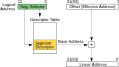
\includegraphics[scale=0.9]{img/segmentacion.pdf}
    \end{center}
\end{frame}

\begin{frame}
    \frametitle{Selector de Segmento}
    \begin{center}
    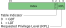
\includegraphics[scale=1]{img/selector_segmento.pdf}
    \end{center}
    \begin{itemize}
        \setlength\itemsep{0.2em}
        \item[] \texttt{CS}: Para acceder a código
        \item[] \texttt{SS}: Para acceder a pila
        \item[] \texttt{DS}: Para acceder a datos (default)
        \item[] \texttt{ES}: Para acceder a datos
        \item[] \texttt{GS}: Para acceder a datos
        \item[] \texttt{FS}: Para acceder a datos
    \end{itemize}
\end{frame}

\begin{frame}
    \frametitle{Descriptor de Segmento}
    \begin{center}
    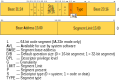
\includegraphics[scale=0.8]{img/descriptor_segmento.pdf}
    \end{center}
\end{frame}

\begin{frame}
    \frametitle{Tipo de Selector de segmento}
    \begin{center}
    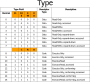
\includegraphics[scale=0.9]{img/segmento_tipo.pdf}
    \end{center}
\end{frame}

\begin{frame}[plain]
    \begin{center}
    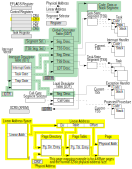
\includegraphics[scale=0.50]{img/usted_esta_aqui.pdf}
    \end{center}
\end{frame}

\begin{frame}
    \frametitle{Pasar a modo protegido}
    \begin{textblock}{100}(21,13)
    \only<1->{\includegraphics[scale=0.44]{img/cataplum-layer1.pdf}}
    \end{textblock}
    \begin{textblock}{100}(21,13)
    \only<2->{\includegraphics[scale=0.44]{img/cataplum-layer2.pdf}}
    \end{textblock}
\end{frame}

\begin{frame}[fragile]
    \frametitle{Pasar a Modo Protegido - ¿Por qué cataplum?}
    \begin{itemize}
    \setlength\itemsep{1.5em}
    \item[] \textcolor{verdeuca}{¿Cómo sabemos donde esta la \texttt{GDT}?}\\
    \pause
    Cargar el registro \verb|GDTR| utilizando \verb|LGDT|
    \item[] \textcolor{verdeuca}{¿Qué tiene la \texttt{GDT}?}\\
    \pause
    Al menos, un descriptor nulo, un descriptor de código y uno de datos
    \item[] \textcolor{verdeuca}{¿Cuál es la próxima instrucción a ejecutar?}\\
    \pause
    La instrucción en la dirección \verb|CS:EIP|
    \item[] \textcolor{verdeuca}{¿Qué valor tiene que tener \texttt{CS} y cómo lo cambiamos?}\\
    \pause
    \verb|..... ; esto se ejecuta en modo real|\\
    \verb|jmp 0x08:modoprotegido|\\
    \verb|; GRAN SALTO!|\\
    \verb|modoprotegido:|\\
    \verb|.... ; esto se ejecuta en modo protegido|
    \end{itemize}
\end{frame}

\begin{frame}[fragile]
    \frametitle{Pasar a Modo Protegido - Pasos}
    \begin{enumerate}
    \setlength\itemsep{1em}
     \item[0-] Completar la \verb|GDT|
     \item[1-] Deshabilitar interrupciones (\verb|CLI|)
     \item[2-] Cargar el registro \verb|GDTR| con la dirección base de la \verb|GDT|\\
                \hspace{1cm}\verb|LGDT <offset>|
     \item[3-] Setear el bit \verb|PE| del registro \verb|CR0|\\
                \hspace{1cm}\verb|MOV eax,cr0|\\
                \hspace{1cm}\verb|OR eax,1|\\
                \hspace{1cm}\verb|MOV cr0,eax|
     \item[4-] \verb|FAR JUMP| a la siguiente instrucción\\
                \hspace{1cm}\verb|JMP <selector>:<offset>|
     \item[5-] Cargar los registros de segmento (\verb|DS|, \verb|ES|, \verb|GS|, \verb|FS| y \verb|SS|)
    \end{enumerate}

\end{frame}

\begin{frame}[plain]
    \begin{textblock}{100}(0,12)
    \uncover<1->{
\includegraphics[scale=0.36]{img/IKnowKungFu.jpg}}
    \end{textblock}
    \begin{textblock}{100}(0,12)
    \uncover<1->{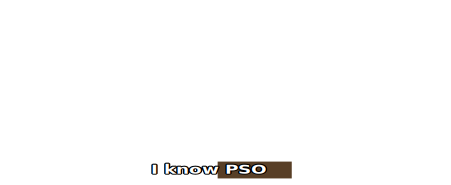
\includegraphics[scale=0.36]{img/IKnowPSO.pdf}}
    \end{textblock}
    \begin{textblock}{55}(3,85)
    \scriptsize
    \texttt{Fuente: Pelicula Matrix}
    \end{textblock}
\end{frame}

\begin{frame}[fragile]
    \frametitle{Bibliografía: Fuentes y material adicional}
    \begin{itemize}
    \item Convenciones de llamados a función en x86: \\
    \url{https://en.wikipedia.org/wiki/X86_calling_conventions}
    \item Notas sobre System V ABI: \\
    \url{https://wiki.osdev.org/System_V_ABI}
    \item Documentación de NASM: \\
    \url{https://nasm.us/doc/}
    \item Artículo sobre el flag \texttt{-pie}: \\
    \url{https://eklitzke.org/position-independent-executables}
    \item Documentación de System V ABI: \\
    \url{https://uclibc.org/docs/psABI-x86_64.pdf}
    \item Manuales de Intel: \\
    \url{https://software.intel.com/en-us/articles/intel-sdm}
    \end{itemize}
\end{frame}

\begin{frame}[plain]
\begin{center}
\vspace{2cm}
\huge ¡Gracias!\\
\vspace{2cm}
\normalsize Recuerden leer los comentarios al final de \\ este video por aclaraciones o fe de erratas.
\end{center}
\end{frame}

\end{document}
